\documentclass[a4paper,11pt,phdthesis,singlespace,twoside]{cssethesis}

\usepackage{harvard} % Use the Harvard bibliography and citation package
\usepackage{graphicx}
\usepackage{epstopdf}
\usepackage{mathptmx}
\usepackage{times}

\usepackage{algorithm}
\usepackage{enumitem}
\usepackage{listings}
\usepackage{color}
\usepackage{apacite}
%\usepackage[backend=biber,style=apa,babel=other,maxcitenames=3]{biblatex}
\usepackage{multirow}

\thesisauthor{Viet Vo}
\thesisauthorpreviousdegrees{BSc., MSc.} % Optional
\thesisdepartment{Caulfield School of Information Technology}
\thesisauthorstudentid{26356988} % Needed for litreview
\thesisauthoremail{viet.vo\@@monash.edu} 

%\thesismonth{October} % Optional. Current month is used if this is not set
%\thesisyear{2015} % Optional. Current year is used if this is not set
\thesistitle{The Effects of Group Member's Parameters on Human Crowd Modelling}
\thesissupervisor{Prof. Bernd Meyer}
\thesissupervisoremail{bernd.meyer\@@monash.edu} 
\thesisassocsupervisor{Dr. Aldeida Aleti} 
\thesisassocsupervisoremail{aldeida.aleti\@@monash.edu} 

% start the document
\begin{document}

\frontmatter					% start the thesis front matter.

\thesistitlepage				% Generate the title page.
%\thesiscopyrightpage			% Generate the copyright page.
%\thesisdedicationpage			% Generate a dedication page (optional)
\tableofcontents				% Generate a table of contents.
\listoftables					% Generate a list of tables (optional).
\listoffigures					% Generate a list of figures (optional).

\begin{thesisabstract}			% generate the abstract page.
This thesis introduces 
\end{thesisabstract}                 

%\thesisdeclarationpage			% generate the declaration page (optional).

%\begin{thesisacknowledgments}	% generate the acknowledgements page (optional).
%I would like to thank everyone who helped to make this possible. It has
%been an incredible journey of self-discovery, and I love every last one of
%you\ldots
%\end{thesisacknowledgments}   

%%%%%%%%%%%%%%%%%%%%%%%%%%%%%%%%%%%%%%%%%%%%%%%%%%%%%%%%%%%%%%%%%%%%%%%%%%%%%%
%%
%% Main matter 
%%
\mainmatter						% start the thesis body.

\chapter{Introduction}
Since over 70\% of the world population is predicted to live in cities by 2050 \cite{Weidmann2012}, rapid urbanization and population growth will be inevitable challenges in the effort of planning infrastructure, estimating traffic needs and capacities, and increasing the safety of pedestrians. With the increase in the number of public events and the number of accidents during these events since the crush disaster happened at the Station Nightclub, USA (2003) \cite{Evers2011}, the demand for realistic crowd simulation models becomes important for risk management in urban design and crowd safety. To develop realistic simulation models, various studies have been conducted in order to understand and simulate behaviours which can emerge in both normal and emergency situations such as groups of pedestrians moving with or competing against each other.

Group cohesion behaviour is the behaviour of objects moving towards the average positions of their neighbors over the time \cite{Reynolds1987}. The definition of this behaviour was motivated by the visual observation of coherently flying objects. The behaviour has been investigated widely on the collective motion of different flocking organisms including homing pigeon flocks \cite{Kattas2012}, fish schools \cite{Miller2013}, and bacteria colony \cite{Cisneros2007}. 

Human group cohesion behaviour is observed by its cohesion degree and formation. Cohesion degree denotes the average distance to the group’s centre of mass from each group member while observable human group formations are V-like, line-abreast, U-like, or river-like \cite {Helbing2005}. Group cohesion behaviour is important in both normal and evacuation scenarios. In normal situations, group cohesion behaviour can affect the speed and movement direction of pedestrians who are not belonging to any group. In human behaviour research, the frequency of group cohesion behaviour’s occurrence has been observed at different places in the UK with the percentages of 37\% at train station, 50\% at shopping centre, 28\% at university campus, 50\%, at Clumber Street \cite{Singh2009}. Pedestrians in the same group might be family members, colleagues. In crowd disasters, pedestrians evacuate with group rather than escape individually. Groups of families and friends with strong ties, stay together and evacuate together have been emphasized through socio-psychological research area \cite {Mawson2005}. They may move irrationally to maintain its cohesion and consequently become obstacles for other pedestrians \cite{Aguirre2011}.

Various models have been constructed to understand group cohesion behaviour such as the cellular automata model, the social-force based model, the standard Vicsek model. These models mainly investigate how model’s outputs which are group’s formation, cohesion degree, and speed change when group population size varies, or explore the collective behaviour of flocking organisms at randomly chosen values of model’s parameters. However, they have not investigate systematically model’s input parameters to explore the most influential parameters which control group information, and how group cohesion affect individuals to make them maintain group cohesion. Yet, the impact of group cohesion behaviour caused by model’s parameters on flow rate which is a crucial measurement of crowd modelling also has not been studied in current studies. Therefore, this PhD study aims to resolve these two research gaps by using systematic analysis methods and proposed simulation scenarios when considering group is the collection of members have the same scalar parameter value or different parameter distributions. This work is to advance our knowledge about model’s the most influential parameters for improving real-time prediction systems and calibration works based on these models, and the impact of group cohesion on flow rate measurement for predicting empty and occupied space for evacuation plan.

Chapter 2 of this report represents the state of the art from models trying to understand group cohesion behaviour. Chapter 3 analyses the drawbacks of current models and presents the need of this research study. Chapter 4 presents proposed research questions. Chapter 5 presents research methodology to resolve these questions. Chapter 6 reports the contribution of this study. Chapter 7 reports current working progress and research timeline to answer these questions. Finally, Chapter 8 outlines compulsory research training hours undertaken in the IT faculty.

\chapter{Literature Review}

This chapter reviews current models that have been constructed to understand group cohesion behaviour. Modelling approaches are various from modelling the changes of each cell on a grid layout, investigating social forces that affect each pedestrian’s acceleration, to providing standard Vicsek model which has been applied widely in flocking organisms with fewer parameters to simulate group members.

\section{Cellular automata model for group behaviour}
Cellular automata-based group behaviour model is the approach relying on Von Neumann's idea that divides space into uniform grid or hexagonal cells. At each time \textit{t}, variables at each cell are updated according to a set of local rules or its neighbour cells. Common local rules are moving direction, or avoidance rules. Every cell in the space can be in different states including free, an obstacle, or occupied by a pedestrian. General cellular automate model is formed as formulas (2.1-2.3).
\begin{equation}
Env = c_{0},c_{1},c_{2},c_{3,},\ldots where\/ \forall c_{i} \in \tetit{Cell}
\end{equation}
\begin{equation}
neighbours(c) = {(c),S(c),E(c),W(c),NE(c),SE (c),NW(c),SW(c)}
\end{equation}
\begin{equation}
State(c)= s \in \left \{Free,Obstacle,Pedestrian_{i}\right \}
\end{equation}
Every cell has variables of path field, obstacle field, and density field. Path field is to identify distance from current cell to destination cell. Obstacle field indicates for every cell the distance from an obstacle or a wall. Density field is to indicate for each cell the crowd density in the surroundings at the current time step t. When running a CA-based pedestrian model, there is several update strategies including parallel update, sequential update, or shuffled sequential update. 

To simulate group behaviour, \cite{Bandini:2011} constructed pedestrians on these defined cells. A pedestrian is represented as a utility-based agent having following attributes:
\begin{equation}
Pedestrian: (Id,GroupId,State,Actions,Destination)
\end{equation}
where:
\begin{itemize}
  \item Id\textendash identification number of pedestrian \textit{i}
  \item GroupId\textendash identification number of group that pedestrian \textit{i} belongs to
  \item State\textendash represents pedestrian’s current cell that and direction followed in last movement
	\item Actions\textendash the set of possible actions to choose an appropriate cell from equations (2.5) and (2.3)
	\item Destination\textendash reflects current path field of the cell where pedestrian i is in
\end{itemize}
An utility function \begin{math}U_{t}(c)\end{math}  was proposed by the author as in equation (2.5). The function estimates the probability of cell \textit{c} to allow pedestrian \textit{i} move in to maintain group cohesion at each time step \textit{t}.
\begin{equation}
U_{t}(c)= \frac{k_{g}G(c)+k_{ob}Ob(c)+k_{s}S(c)+k_{d}D(c)+k_{ov}Ov(c)+k_{c}C_{i}(c)+k_{i}I_{i}(c)}{d}
\end{equation}
where:
\begin{itemize}
  \item $ \begin{math} \textit{k_{g}}, \textit{k_{ob}}, \textit{k_{s}},\textit{k_{d}},\textit{k_{ov}},\textit{k_{c}},\textit{k_{i}}  \in [0,100] \end{math} $ are model's parameters for their corresponding functions 
	\item  \begin{math} G(c)\end{math} is the goal attraction derived from current cell's path field and destination cell's path field 
	\item  \begin{math} Ob(c)\end{math} represents obstacle repulsion from obstacle field of current cell c over the maximum distance to obstacles from any cell in grid layout 
	\item  \begin{math}S(c)\end{math} represents separation value to allow pedestrian i avoid other pedestrians. It is measured by density field of current cell c over the predefined maximum density 
	\item \begin{math}D(c)\end{math} represents whether this cell is the same direction with previous movement of pedestrian 
	\item \begin{math}Ov(c)\end{math} represents a small probability to allow two pedestrians stay on the same cell
	\item \begin{math}C_{i}(c)\end{math} represents cohesion value of cell \textit{c} if pedestrian \textit{i} move in towards other group member's position
	\item \begin{math}I_{i}(c)\end{math} is used in the case of large group which can be separated into sub groups. It represents the cohesion value of current pedestrian toward the largest group
	\item \textit{i} is the distance from cell \textit{c} to pedestrian \textit{i}'s current cell position. d is only equal to 1 or \begin{math} \sqrt{2} \end{math}
\end{itemize}	
Group cohesion degree is then defined as in equation (2.6) to represent the average distance from each group member to group's centre of mass. The study used this degree to support pedestrian \textit{i} trade off current goal attraction with group cohesion based on predefined rules.
\begin{equation}
Cohesion(Group)= \frac{\sum_{\substack{i=1}}^{Size(Group)}distance(centroid,a_{i})}{Size(group)}
\end{equation}
The study then measured the correlation between group size and group cohesion speed in various design layouts. However, this CA-based model only allows pedestrians move in neighbour cells rather than in further cells at each time step. It applied the same value of each parameter \begin{math} \textit{k_{g}}, \textit{k_{ob}}, \textit{k_{s}},\textit{k_{d}},\textit{k_{ov}},\textit{k_{c}},\textit{k_{i}}  \in [0,100] \end{math} for whole group members. Group speed and cohesion degree are investigated when group population size varies; specifically, group speed decreases when increasing population size. However, the effect of these parameters on group degree and the impact of group cohesion behaviour on flow rate measurement were not investigated by its authors.

\section{Social force model for group behaviour}
Moussaid, Helbing and colleagues \cite{Moussaid2010} created the social group-force model based on the social-force model \cite{Helbing1995} \cite{Helbing2000}. The social group model (equation 2.7-2.8) represents that a pedestrian \textit{p} at time \textit{t} is trying to move with a certain desired speed \begin{math} \textit{v_{p}^{d}(t)} \end{math} in a desired direction \begin{math} \textit{\vec{e}_{p}^{\,d}(t)}\end{math} pointing from pedestrian \textit{p}'s current position to his target position . Therefore, pedestrian \textit{p} tends to correspondingly adapt his actual velocity \textit{\vec{v}_{p}(t)}\end{math} with a certain acceleration time \begin{math}  \tau_{p} \end{math}. The acceleration time represents pedestrian \textit{p} changes its current velocity and return to its desired velocity. Pedestrian \textit{p}'s acceleration at time \textit{t} is also influenced by repulsive forces coming from surrounding pedestrians and obstacles. They are \begin{math} \sum_{\substack{\textit{q}\neq(\textit{p})}}\vec{f}_{\textit{pq}}(\textit{t}) \end{math} and \begin{math} \sum_{\gamma}\vec{f}_{\textit{p\gamma}}\end{math} (\textit{t})  respectively. The repulsive force’s directions and group force direction are represented in Figure~\ref{fig:repulsive_force}. The group influence force \begin{math} \vec{f}_{p}^{group}(t)\end{math} aims to describe that an individual in group continuously adjusts its position to reduce its head direction and maintain group's centre of mass, but also avoid other group members. The group force is represented in equation 2.9.
\begin{equation}
\frac{d\vec{v}_{p}(t)}{dt}= \vec{f}_{p}(t) + \xi_{p}(t)
\end{equation}
\begin{equation}
\vec{f}_{p}(t)= \frac{1}{\gamma}_{p}}\left(v_{p}(t)\vec{e}_{p}^{\,d}(t) - \vec{v}_{p}(t) \right) + \sum_{\substack{\textit{q}\neq(\textit{p})}}\vec{f}_{\textit{pq}}(\textit{t}) + \sum_{\gamma}\vec{f}_{\textit{p$\gamma$}}(t) + \vec{f}_{p}^{group}(t)
\end{equation}
where \begin{math} \textit{v_{p}^{d}(t)} \end{math} is the desired speed of pedestrian p that varies over time, \begin{math} \xi_{p}(t)\end{math} is an uncertainty factor. 
\begin{equation}
\vec{f}_{p}^{group}(t)= \vec{f}_{p}^{vis}(t) + \vec{f}_{p}^{att}(t) + \vec{f}_{p}^{rep}(t)
\end{equation}
\begin{figure}[ht]
\begin{center}
\resizebox{100mm}{!}{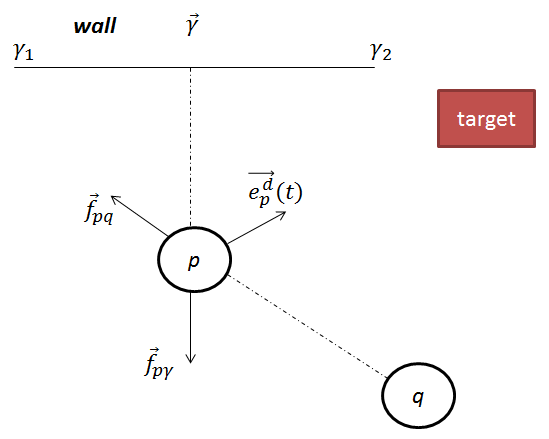
\includegraphics[width=0.05\columnwidth]{figs/repulsive_force.png}}
\end{center}
\caption{Repulsive forces \begin{math}\vec{f}_{\textit{pq}} \end{math} and \begin{math}\vec{f}_{\textit{p$\gamma$}} \end{math} on pedestrian \textit{p} created by pedestrian \textit{q} and wall \gamma}
\label{fig:repulsive_force}
\end{figure}	
The social group force \begin{math}\vec{f}_{p}^{group}(t) \end{math}describes that pedestrian \textit{p} at time \textit{t} turns his gazing direction to see their partners. Thus, \begin{math} \vec{f}_{p}^{vis}(t)\end{math} vision force is included to help pedestrian \textit{p} adjust its position to reduce the head rotation. At the same time, pedestrian \textit{p} keeps a certain distance to the group's centre of mass by the force \begin{math}\vec{f}_{p}^{att}(t)\end{math}. A repulsive force\begin{math} \vec{f}_{p}^{rep}(t)\end{math} is added to support pedestrian \textit{p} avoid other group members. These group element forces are presented in equations (2.10-2.12).
\begin{equation}
\vec{f}_{p}^{vis}(t) = -\beta_{1}\alpha_{p}\vec{V}_{p}(t)
\end{equation}
\begin{equation}
\vec{f}_{p}^{att}(t) = -q_{A}\beta_{2}\vec{U}_{p}(t)
\end{equation}
\begin{equation}
\vec{f}_{p}^{rep}(t) = \sum{\substack{k}}q_{R}\beta_{3}\vec{W}_{pk}(t)
\end{equation}
where:
\begin{itemize}
  \item $\beta_{1}$ is the model's parameter describing the strength of the social interactions between group members
	\item $\alpha_{p}$ is the angle constructed by the vector pointing to target direction and current gazing direction. The angle varies from 0 degree to maximum angel constructed by the target direction and the vector point from pedestrians \textit{p}'s current position to group centre of mass at time \textit{t}. The larger angel $\alpha_{p}$ means that pedestrian \textit{p} feels less comfortable to move and consequently reduce his speed at time \textit{t}. The angle $\alpha_{p}$ is represented in Figure~\ref{fig:alpha_vision}.
\begin{figure}[ht]
\begin{center}
\resizebox{80mm}{!}{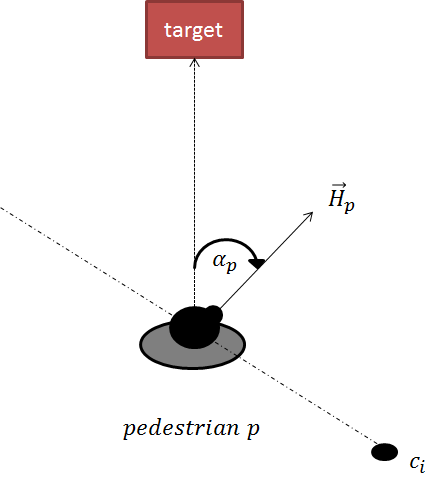
\includegraphics[width=0.05\columnwidth]{figs/alpha_vision.png}}
\end{center}
\caption{Pedestrian \textit{p} turns his gazing direction \begin{math}\vec{H}_{p}(t) by an angel \alpha_{p} to see their group centre of mass c_{i}}
\label{fig:alpha_vision}
\end{figure}	
	\item $\beta_{2}$ is model's parameter describing the strength of the attraction effects
	\item  \begin{math}\vec{U}_{p} \end{math} is the unit vector pointing from pedestrian p to the centre of mass
	\item $q_{A}=1$ if the distance between pedestrian p and group centre of mass exceeds the threshold \begin{math}\frac{N-1}{2} \end{math} meters
	\item $\beta_{3}$ is the model's parameter describing the repulsion strength between group members
	\item $q_{R} = 1$ if pedestrians \textit{p} and \textit{k} overlap each other; otherwise, $q_{R} = 0$
	\item \begin{math}\vec{W}_{pk}\end{math} is the unit vector pointing from pedestrian \textit{i} to the group member \textit{k} 
\end{itemize}	
To summary, the social force model comprises parameters that need to be set at initial simulation time as in Table~\ref{tab:model_params}.

\begin{table}[H]
\caption{Social-group force model's parameters}
\begin{tabular}{|l|l|l|} \hline
\textbf{Parameter} & \textbf{Component} & \textbf{Description} \\ \hline
$ V_{p}^{Id}$ &Desired Acceleration& Initial desired velocity \\ \hline
$ \gamma_{p}$ &Desired Acceleration& Acceleration time \\ \hline
$\texit{c}$ &Desired Acceleration& Constant to find maximum velocity  \\ \hline
$ \textit{A}$ & Repulsive Force with other pedestrians& Interaction strength \\ \hline
$ \textit{B}$ & Repulsive Force with other pedestrians& Interaction range \\ \hline
$ \textit{U}$ & Obstacle Force & Obstacle interaction strength  \\ \hline 
$ \textit{R_{p}}$ &  Simulation & Radii of pedestrian \textit{p}\\ \hline 
$ \beta_{1}$ &  Group vision force & The strength of the social interactions\\ \hline 
$ \beta_{2}$ &  Group attraction force & The strength of the attraction effects \\ \hline 
$ \beta_{3}$ &  Group repulsion force & The repulsion strength between group members\\ \hline 
\end{tabular}
\label{tab:model_params}
\end{table}
Social-force based model has possessed a long-life modification period by its author and colleagues for more than a decade in order for simulating the additional factors affecting individual's acceleration or being easier towards calibration process. However, it almost uses the same parameter distribution to simulate pedestrians inside crowd as in Table~\ref{tab:model_params_values}.
\begin{table}[H]
\caption{Social-group force model's parameter values}
\begin{center}
\begin{tabular}{|l|l|l|} \hline
\textbf{Parameter} & \textbf{Value} & \textbf{Reference} \\ \hline
\multirow{2}{*}{$ V_{p}^{Id}(m/s)$}& avg. = 1.34, st. dev. = 0.26 & \cite{Helbing1995}\\ 
															& avg. = 1.3, st. dev. = 0.3 & \cite{Helbing2005} \\ \hline
\multirow{2}{*}{$ \gamma(s)$}& 0.5 & \cite{Helbing1995}\\ 
															& 0.1 & \cite{Helbing2000} \cite{Helbing2005}\\ \hline
\textit{c}&1.3&\cite{Helbing1995} \cite{Helbing2000} \\ \hline
\textit{A}(m/s^{2})&3.0 &\cite{Helbing2005}\\ \hline
\textit{B}(m)&0.2&\cite{Helbing2005}\\ \hline	 																										
\end{tabular}
\end{center}
\label{tab:model_params_values}
\end{table}
Through actual observation, Moussaid found that pedestrians in the same group likely move in a line-abreast formation to allow them communicate with each other easily. When crowd density increases, group of pedestrians automatically change its formation into V-shaped or river-like pattern. According to the study, when the model parameter $\beta_{1}=0$, it shows that group members only try to stick together with no communication rule. When $\beta_{1}=4$, a V-shaped structure is created. 

The authors applied the same value of each parameter in Table~\ref{tab:model_params_values} and parameters of group force $\beta_{1}, \beta_{2}, \beta_{3}$ to all pedestrians inside group to see these patterns. In fact, human group formation is various from V-line, U-like, line-abreast, to river-abreast as in actual observation (Helbing, 2005). However, this model did not mention at which values of parameters $\beta_{1}, \beta_{2}, \beta_{3}$ other group formations could be created. It also raises a question whether these parameters have to be the same for all group members to establish these structures. Similar with CA-based model, the authors of social-group force models have not investigated the effect of member’s parameters (e.g. $ V_{p}^{Id}, \gamma, \textit{A}, \textit{B} $) on group speed and formation. They only studied how these information change according to different group population sizes; specifically, they found that group speed decreases when group population size increases. 

\section{Standard Vicsek model of flocking organisms}
In order to interpret the behaviour of huge flocks of living organisms (flock of birds, fish schools, and bacterium, and human crowd) in the presence of perturbations, a statistical physic approach has been introduced to the flocking by Vicsek \cite{Vicsek1995}. Nowadays, it has been called as Standard Vicsek Model as suggestion of \cite{Huepe2008}. The model considers that self-propelled particles represent living flocks, and perturbations are natural consequence of stochastic and deterministic factors affecting the motion of particle. The model is presented in equations (2.13-2.14).
\begin{equation}
\vec{v}(t+1)= \vec{v}_{0}\frac{\langle\vec{v}_{j}(t)\rangle_{R}}{|\langle\vec{v}_{j}(t)\rangle_{R}|} + \textit{perturbations}
\end{equation}
\begin{equation}
\vec{x}(t+1)= \vec{x}(t) + \vec{v}(t+1)
\end{equation}
The main idea of the model is that at each given time step \textit{t}, particle \textit{i} is usually controlled by interactions with its local neighbors in a constant radius \textit{R} and uncertainty factor perturbations. Here \begin{math}\langle\vec{v}_{j}(t)\rangle_{R} \end{math} denotes the averaging of the velocities of neighbours in radius \textit{R}. The expression \begin{math} \frac{\langle\vec{v}_{j}(t)\rangle_{R}}{|\langle\vec{v}_{j}(t)\rangle_{R}|}\end{math} provides a unit vector pointing in the average direction of motion. The particle \textit{i} also has a constant velocity \begin{math} \vec{v}_{0} \end{math}. In the standard version of the model, Vicsek derived the perturbations factor by adding a random angle to the angle corresponding to the average motion direction of particle \textit{i}'s neighborhood. The angel \begin{math} \vartheta_{i} \end{math} of average motion direction and random angle $\Delta_{i}$ at time \textit{t} are represented as in equations (2.15-2.16).
\begin{equation}
\vartheta_{i}(t)= \tanh\left(\frac{\langle v_{j,x}\rangle_{R}}{\langle v_{j,y}\rangle_{R}}\right)
\end{equation}
\begin{equation}
\vartheta_{i}(t+1)= \vartheta_{i}(t) + \Delta_{i}(t)
\end{equation}
where \begin{math}  v_{j,x} and  v_{j,y} \end{math} are the x and y coordinates of particle \begin{math} \textit{j^{th}}'s \end{math}velocity in the neighborhood of particle \textit{i}. The perturbation $\Delta_{i}(t)$ s a random number taken from uniform distribution in the interval $[-\eta\pi,\eta\pi ]$. The randomness of perturbation makes particles have different motion direction from those of others. The velocity $ \begin{math} \textit{v_{0}} \end{math} $ was set the same for all birds in flocks. Finally, two control parameters of the model are the density $ \rho $ (number of particles in a volume $ \begin{math} \textit{R^{d}} ( \textit{d}  \end{math}$  is the dimension)), and the level of perturbation $\begin{math} \eta \end{math} $.

In the studies of the authors \cite{Vicsek1995}\cite{Czirok2000}, the average momentum of the particles \begin{math}\phi \equiv \frac{1}{N}|\sum_{j}\vec{v}_{j}| \end{math} and the correlation between particles' velocity directions were investigated when varying model's parameters including the level of perturbation, the density $ \rho $ , and population size. In these studies, the author considered the density ρ at the values 2, 4, 0.5 and explored the average momentum at corresponding values of the level of perturbation $\eta$ at 1,2,3,4,5. The author found that the average momentum decreases when decreasing the density or increasing the level of perturbation. 

There is also another approach from the author to investigate the role of model's parameters \cite{Bhattacharya2010} on group cohesion behaviour. This study derived the model in 3D dimensional environment to explore the cohesiveness through the process of landing of bird flocks performing foraging flights. The study explored the heterogeneity in attributes such as the ages, sex, and social status of animals in group or the differences in the perception of external stimuli by assigning to each bird $ \textit{i} $  an inherent switching time $\begin{math} \textit{t_{i}} \end{math}$, such that if the bird begins a flight at time $ \textit{t}=0 $, it would decide to land at time  $ \begin{math}\textit{t}= \textit{t_{i}} \end{math}$.This work was to show that the difference in the attributes implied the difference in energy reserve to maintain an altitude.\begin{math} \text{t_{i}}'s \end{math} was selected from a Gaussian distribution with a given standard deviation $\sigma_{0}$. The study then investigated quantitatively the fraction of birds not landed yet as time $ \textit{t} $ progresses when setting to different \begin{math}\sigma_{0} \end{math} values. However, the model's parameters $\begin{math}\rho ,\eta, \textit{v_{0}} \end{math}$ were set the same for all birds $ \begin{math}(\rho = 2.0, \eta=0.2, \textit{R}=2.0, \textit{v_{0}}= 0.01) \end{math}$.

In summary, standard Vicsek model used the particle-based approach to understand flocking organisms. The author's proposed studies investigated collective behaviour when varying model's parameters arbitrarily, adding a new constraint for landing period of individual group members to simulate the heterogeneity of group members. However, these studies have not yet explored systematically the effect of parameters to find the most influential parameters on collective behaviour. Moreover, these studies also have not yet considered flock of individual group members who have different parameter distributions to those of others in these parameters.


\chapter{Figures and Tables}
Here we will test that references to figures and tables work correctly.

\section{Figures}
\begin{figure}[H]
\begin{center}
\resizebox{100mm}{!}{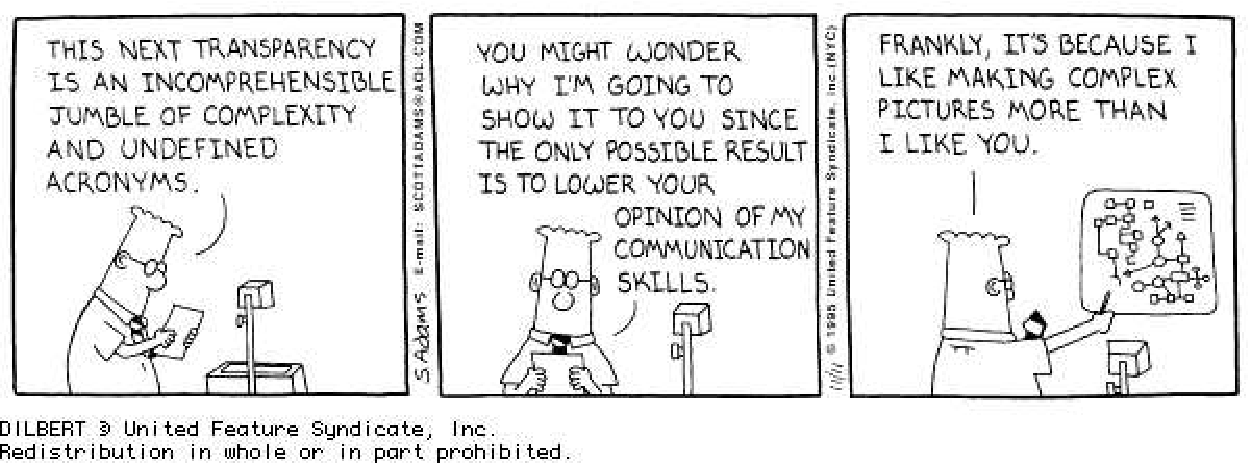
\includegraphics{dilbert_complexpictures}}
\end{center}
\caption{An example of a figure.}
\label{fig:example}
\end{figure}
See Figure~\ref{fig:example}.

\section{Tables}
\begin{table}
\begin{center}
\begin{tabular}{lcr}
23121 & 1212 & 232 \\ \hline  
cat & frog & dog
\end{tabular}
\end{center}
\caption{An example of a table}
\label{tab:example}
\end{table}
See Table~\ref{tab:example}.

\subsection{Referencing test}
See Table~\ref{tab:example} and Figure~\ref{fig:example}.


\begin{figure}[ht]
\begin{center}
\resizebox{100mm}{!}{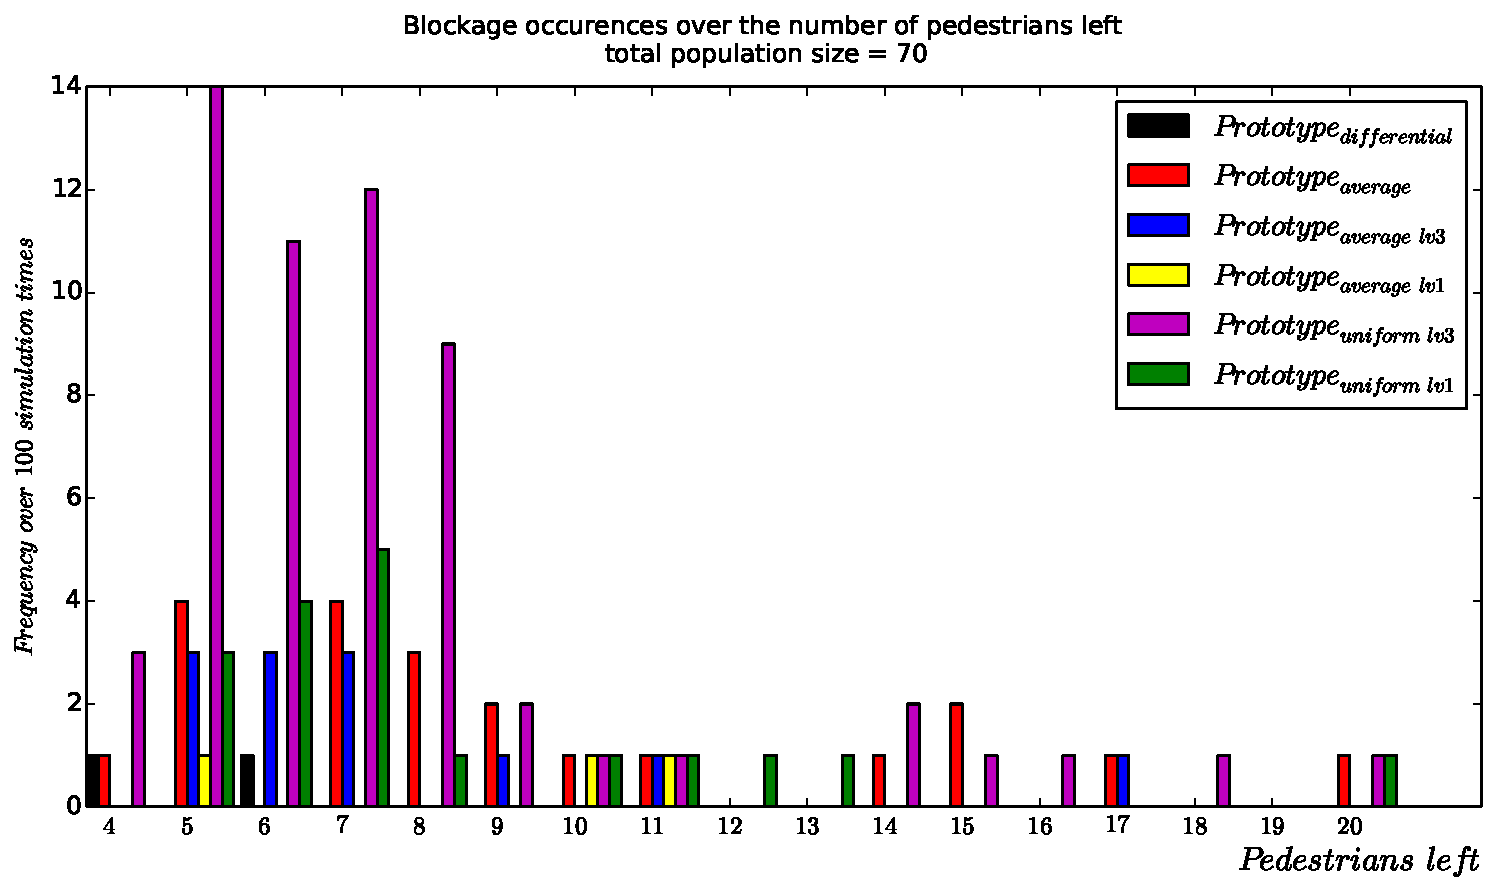
\includegraphics[width=0.05\columnwidth]{figs/blockage_frequency.pdf}}
\end{center}
\caption{An example of a figure.}
\label{fig:example}
\end{figure}

\appendix % all \chapter{..} commands after this will generate appendices

\chapter{This appendix should get a letter}
\label{app:example}
An appendix before the backmatter gets an automatically generated letter by
which it can be referred to. This is Appendix~\ref{app:example}.

\chapter{Simulation Source Code}
You may want to investigate the \texttt{lgrind} program and package if you
wish to include source code in your thesis

%%%%%%%%%%%%%%%%%%%%%%%%%%%%%%%%%%%%%%%%%%%%%%%%%%%%%%%%%%%%%%%%%%%%%%%%%%%%%%
%%
%% Back matter 
%%

\backmatter						% start the thesis back matter
\bibliographystyle{apacite}
\bibliography{confirmationmonashbib}

\chapter{Last Thing} 
This sort of appendix has no letter. 


\end{document}
